\documentclass{article}
\usepackage[margin=1.5cm]{geometry}

\usepackage{tikz}
\usepackage{amsmath}
\usepackage{tcolorbox}
\usepackage[utf8]{inputenc} %svenska symboler
\setlength\parindent{0pt} %Ingen indent

\author{Fredrik Jansson}
\date{\today}
\title{Komplex Analys}



\begin{document}

\maketitle

\section*{Sammanfattning}
Komplex analys är en av de svåraste kurserna på utbildningen Teknisk Fysik. Enligt statestiken på (https://ysektionen.se/student/tentastatistik/tata45/). Det följer att detta är något som man måste lägga tid på för att klara. Jag har bestämt mig för att göra en sammanfattning. Sammanfattningen ska handla om attförklara nyckelkoncept och vara ett lösningsförslag till typuppgifter. 


\section{Beräkna Antalet Nollställen}
Detta är en väldigt vanlig uppgift på tentan, vad jag kan se så har den varit med på alla tentor som ligger ute. Uppgiften brukar vara formulerad ungefär såhär 
Här är annan text. 
\begin{tcolorbox}
Bestäm antalet nollställen som polynomet 
\begin{align*}
	p(z) = ...
\end{align*}
har i området ... (oftast ett halvplan)
\end{tcolorbox} 


Ett spciallfall som kan vara värt att undersöka är ifall $p(z)$ har något nollställe som är rent reelt eller rent imaginärt och om detta ligger på $L_R$ eller $I_R$. Om så är fallet så ingår inte denna i området och man behöver faktorisera bort detta nollställe innan man börjar sina beräkningar. Man kommer då att få ett polynom $q(z)$ som är minst en grad mindre än $p(z)$ vilket är det polynom man ska göra resterande beräkningar på. 

\subsection{Antal Nollställen I Halvplan/Kvadrant }
Det första steget är att rita upp situationen. Man gör detta genomom att beskriva området som en tårtbit.
\begin{center}
\begin{tikzpicture}
	\draw[->] (0,0) -- (1.5,0);
	\draw[->] (0,0) -- (0,1.5);
	\draw[->] (0,0) -- (-1.5,0);
	\draw[->] (0,0) -- (0,-1.5);
	\draw[very thick] (0,1) arc (90:0:1);
\end{tikzpicture}
\qquad
\begin{tikzpicture}
	\draw[->] (0,0) -- (1.5,0);
	\draw[->] (0,0) -- (0,1.5);
	\draw[->] (0,0) -- (-1.5,0);
	\draw[->] (0,0) -- (0,-1.5);
	\draw[very thick] (-1,0) arc (180:0:1);
\end{tikzpicture}
\qquad
\begin{tikzpicture}
	\draw[->] (0,0) -- (1.5,0);
	\draw[->] (0,0) -- (0,1.5);
	\draw[->] (0,0) -- (-1.5,0);
	\draw[->] (0,0) -- (0,-1.5);
	\draw[very thick] (-1,0) arc (-180:0:1);
\end{tikzpicture}
\end{center}
Där man låter radien, $R \rightarrow \infty$. På detta sätt skapas en tårtbit som täcker in hela området. Det finns konventioner i kursen för hur dessa linjer och bågar ska namnges. Bågelementet kallas $C_R$, sträckan på den realla axeln kallas $L_R$ och sträckan på den imaginära axeln kallas $I_R$. Som man kan se i bilden så är det möjligt att ett område bara har en av dessa sträckor, om vinkeln på bågelementet är $\pi$.

Nästa steg är att nogrant tänka ut riktningen på dessa sträckor och bågar. Dessa riktningar bestämmer tecknet då man ska räkna ut det totala tillskottet som det inneslutna området $\Gamma_R$ utgör. För de tre bilderna ovan får vi
\begin{align*}
	\Gamma_R =& C_R + L_R + I_R \\
	\Gamma_R =& C_R + L_R \\
	\Gamma_R =& C_R - L_R
\end{align*}
Håller man tungan rätt i mun kan man göra detta på flera sätt. Jag föredrar att alltid låta $L_R$ och $I_R$ peka åt höger respektive uppåt, medans $C_R$ alltid har positiv riktning. \\

\subsubsection*{Bågelementets Bidrag}
Nästa steg är att beräkna bidraget som bågelementet utgör. Detta uttrycks
\begin{align*}
	\Delta_{C_R} \arg p(z)
\end{align*}
Vad man ofta uttnyttjar är att operationen $\arg$ har egenskapen 
\begin{align*}
	\arg \left( p(z) g(z) \right) = \arg p(z) + \arg g(z)
\end{align*}
Vad man gör är att bryta ut den största exponeneten. Om man använder ett godtyckligt polynom som exempel får man någos i stil med
\begin{align*}
	\Delta_{C_R} \arg \left( z^3 + 4z^2 + z + 3 \right) = \Delta_{C_R} \arg z^3 + \Delta_{C_R}\arg \left( 1+4/z+1/z^2 + 3/z^3 \right)
\end{align*}

När $R \rightarrow \infty$ så kommer den högra termen att gå mot $\arg 1 = 0$. Så i detta exempel så försvann denna termen helt, vilket den gjort i alla exempel jag undersökt. Nästa steg blir att beräkna termen som är kvar, för detta kan vi använda en annan trevlig egenskap hos $\arg$-operationen.
\begin{align*}
	\Delta_{C_R} \arg z^n = n \Delta_{C_R} \arg z 	
\end{align*}
Vi vet vad n är och $\Delta_{C_R} \arg z$ är helt enkelt argumentet för bågelementet. Nu vet vi bågelemtets tillskot. \\

\subsubsection*{Sträckornas Bidrag}
Nästa steg är att beräkna tillskottet för sträckan eller sträckorna som skapar det inslutna området tillsammans med bågelementet. Om vi går tillbaks till bilden i början avsnittet så finns det här lite olika fall. I den första bilden så behöver två sträckor undersökas. Dessa undersöks separat genom att ersätta $z$ med $x$ respektive $iy$. Man får då två polynom
\begin{align*}
	p(x) = ... = u(x) + iv(x) \\
	p(iy) = ... = u(y) + iv(y)
\end{align*}
\textbf{Fall 1: Bild 1} \\
Detta kanske är det lurigaste fallet, i alla fall om några av konstanterna i polynomet är koplexa. Är de inte det så är i alla fall realdelen tämligen lättberäknad. Vad man behöver göra är att beräkna $\Delta_{L_R + I_R} \arg p(z)$. Som tur är så börjar den ena där den andra slutar, så man kan räkna dem i "serie". I vårat exempel så börjar man med att göra ett teckenstudie för $u+iv$ då $x: R \rightarrow 0$ och för $y:0 \rightarrow R$. Det är då som att man får ett teckenstudie som slutar i 0 och ett som börjar där, på detta vis kan man rita ut kurvan i uv-planet för. Från denna kurva ska man sedan kunna avläsa argumentet för $\Delta_{L_R + I_R}$. \\

\textbf{Fall2: Bild 2 och 3} \\
I dessa fall behöver man bara ansätta ett polynom, $p(x)$ eller $p(iy)$ beroende på om sträckan är horizontel eller vertikal. Sedan gör man om polynomet på formen $u+iy$ och gör teckenstudie mellan $x/y: -R \rightarrow R$. Fråen detta ska man kunna rita kurvan och avläsa argumentet för sträckan. \\

\textbf{Speciallfall, vinkel inte multipel av $\pi/2$} \\
I dessa fall får man göra en parimatisering med en variabel $t$ och ansätta $t+it$ i polynomet, om vinkeln skulle vara $\pi/4$. \\

\subsection*{Sätta Ihop Allt}
Nu har vi kommit till det slutgiltiga steget, att addera alltihop och se reslultatet. Detta brukar uttryckas
\begin{align*}
	\lim_{z \rightarrow R} \frac{1}{2 \pi} \Delta_{C_R + L_R + I_R} \arg p(z)
\end{align*}
Vad detta innebär är att man adderar alla argument man räknat ut innan, eller subtraherar om elementet är negativt, och delar alltihop med $2 \pi$, svaret är antalet nollställen minus antalet poler. \\


\subsection{Antalet Nollställen I En Cirkelskiva}
Detta är också en vanlig uppgift vad gäller beräkning av antalet nollställen i ett område. Det är vanligt att detta är en deluppgift och man använder samma polynom i båda uppgifterna. Det kommer antas att man lånar många koncept från tidigare avsnitt, så allt förklaras inte här. Uppgifter uttrycks ofta något i stil med

\begin{tcolorbox}

Bestäm antalet nollställen som polynomet 
\begin{align*}
	p(z) = ...
\end{align*}

	har på (enhet) skivan $|z| < r$

\end{tcolorbox}
Området får då utseendet. 
\begin{center}
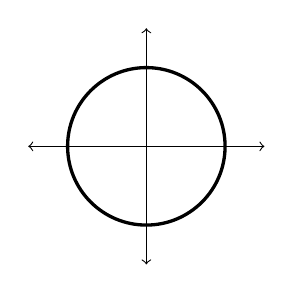
\begin{tikzpicture}
	\draw[->] (0,0) -- (1.5,0);
	\draw[->] (0,0) -- (0,1.5);
	\draw[->] (0,0) -- (-1.5,0);
	\draw[->] (0,0) -- (0,-1.5);
	\draw[very thick] (1,0) arc (360:0:1);
\end{tikzpicture}
\end{center}
Man kan redan börja misstänka att denna kalkyl har med polära koordinater att göra, och det har det. När man löser denna typen av uppgift så ersätter man $z$ med $e^{i \theta}$. Man sätter in detta i polynomet och uttrycker det hela på $u + iv$ -form. Detta steg kräver att man gör om alla termer till cos och sinus, för att kunna dela upp dessa delar. \\

När man delat upp alla delar så görs ett teckenstudie mellan $-\pi$ och $\pi$, där man är noggran med att undersöka alla nollställen på vägen för både u och v. Därefter används argumentprincipen, som i tidigare avsnitt.  

\section{Integraler}
Det finns uppgifter som har att göra med att beräkna integraler. Jag har börajat misstänka att dessas löösningsgång är så olika att det kanske är dumt att ha dem under samma rubrik.

\subsection{Residykalkyl}

\begin{tcolorbox}
Beräkna integralen (med residykalkyl)

\begin{align*}
	\int_{\infty}^{\infty} f(x) dx \quad \text{eller} \quad \int_{0}^{\infty} f(x) dx \quad \text{eller} \quad  \int_{-\pi}^{\pi} f(\theta) d \theta
\end{align*}

\end{tcolorbox}
Dessa integraler beräknas valigtvis med residykalkyl, om uppgiften tvingar en eller inte. Vad man gör först är att rita upp området. Man kan dock vara lite lurig, göra det lätt för sig. \\ 

\textbf{Integral 1} I den första integralen så vill man lägga till ett bågelement i det komplexa talplanet, så man får ett omslutet område. Man kan göra detta på två sätt, man kan lägga båden under eller över realaxeln. När man väler detta så är det viktigt att bågelementets bidrag är ändligt, det får man undersöka med ML-uppskattning och liknande. Om båda går så kan det vara smart att välja att lägga till den som är enklast att räkna ut. Om den ena sidan bara har en pol och den andra har 3 så borde valet vara uppenbart. Om funktionen är jämn så finns ett annat trick, man kan bara räkna ut en kvarts cirkelskiva och gångra med 2. Därefter kan man beräkna residyn och dra bort potentiella tillskott. \\ 

\textbf{Integral 2} Se tidigare fall. Något att tänka på här är att man kan göra tvärt om, om funktionen är jämn så kan man ta en halv cirkelskiva och halvera resultatet. I annat fall akn man tvingas lägga till en sträcka $I_R$, dennas bidrag behöver tas hänsyn till. Därefter kan man beräkna residyn, och dra bort botensiella tillskott.\\ 

\textbf{Integral 3} Här känns polära koordinater rimligt. Man ersätter $\theta$ med $e^{i \theta} = z$ och $d \theta = dz/iz$, därefter kan man beräkna residyn i området.
\\

\subsubsection*{Beräkna residy}
Det säkraste sättet är att göra en serieutveckling, förutsatt att man är ett matematiskt geni så ska detta alltid gå att göra. Man kan använda serieutvecklingar, stora ordo men mer, för att få fram $c_{-1}$-konstanten ur serien, detta är per definition residyn. \\

I vissa fall akn man göra det enkelt för sig själv genom att använda regler som finns att tillgå. Båda dessa bygger på att man vet polerna för $f(z)$, man har då regler
\begin{align*}
	f(z) = \frac{g(z)}{(z-z_0)^N} \iff \underset{z=z_0}{\text{Res}} f(z) = \frac{1}{(N-1)!}\lim_{z = z_0} \frac{d^{N-1}}{dz^{N-1}} \left( (z-z_0)^N f(z)\right)
\end{align*}
Den andra är
\begin{align*}
f(z) = \frac{g(z)}{q(z)} \iff \underset{z=z_0}{\text{Res}}f(z) = \frac{p(z_0)}{q'(z_0)}	
\end{align*}

\subsection{Räkna ut integralen}
Integralen är nu $2 \pi i \cdot (\text{alla residyer i området})$

\subsubsection*{Sammanfattning}

\begin{itemize}
	\item Bestäm rimligt område. Man kan till exempel uttnyttja att funktionen är jämn. Tänk på alla bidrag som läggs till, alla dessa måste konvergera. 
	\item Beräkna residyerna i det valda området. Har man enkelpoler så kan man använda den andra formeln. Är poelen av högre ordning så kan man använda formel 1. Är det inte en pol eller hävbar pol, utan en essentiell, så är serieutveckling enda sättet.
	\item Addera, subtraher och sånt, så man får ut det sökta bidraget. 
\end{itemize}

\subsection{Residykalkyl på Fourierintegraler}


\begin{tcolorbox}
Beräkna integralen (med residykalkyl)

\begin{align*}
	\int_{\infty}^{\infty} h(x) \cdot e^{iax} dx \quad \text{eller} \quad \int_{0}^{\infty} h(x) \cos{ax} dx \quad \text{eller} \quad  \int_{-\pi}^{\pi} h(x) \sin{ax} dx
\end{align*}
\end{tcolorbox}

Lösningsgången på dessa verkar vara väldigt liknande. Skillnaden i stort sett är att man kan nyttja Jordans lämma som säger att
\begin{align*}
	\int_{C_R^+} |e^{iax}| |dx| \leq \frac{\pi}{R}
\end{align*}
När man löser denna typ utav integral så brukar man vilja ha den periodiska funktionen uttryckt i $e^{i x}$. Man kan göra detta enkelt genom att helt enkelt ersätta den periodiska funktionen med detta och ta antingen real eller imaginärdelen av alltihop. 

\subsection{Nyckelhålsstrukturer}
Nyckel.hålsstrukturer är i strort sett en extrapolisering på tidigare nämnt. Skillnaden är att man nu även lägger till en båga, tex kring origo. Man kan på detta sätt undervika en essentiel singularitet och liknande. Skillnaden är att man nu har en till båge, $C_\epsilon$ , vars bidrag är då man låter $\epsilon \rightarrow \infty$.









\section{Bestämma en analytisk funktion.}
Det finns uppgifter där man ska bestämma en hel analytisk funktion $f(z) = u +iv$ givet vad $u+v$ är eller något i den stilen.
\begin{tcolorbox}
	Bestäm alla (hela analytiska) funktioner $f(z) =u+iv$ sådanna att 
\begin{align*}
	u \pm v = f(x,y) \quad \text{och} \quad f(c) = C
\end{align*}
	Sedan ska $f$ uttryckas i $f(z)$.
\end{tcolorbox}
Här gäller det att veta Cochy-kriterierna, nämligen 
\begin{align*}
	\begin{cases}
		u'_x = v'_y \\
		u'_y = -v'_x
	\end{cases}
\end{align*}

\subsection{Derivera $f(x,y)'_x$ och $f(x,y)'_y$}
Detta kommer att skapa två ekviationssystem. 
\begin{align*}
	\begin{cases}
		f(x,y)'_x = u'_x \pm v'_x  = ... \\
		f(x,y)'_y = u'_y \pm v'_y = ...
	\end{cases}
\end{align*}

\subsection{Lös ut $u'_x$ och $u'_y$ eller $v'_x$ och $v'_y$}
Man kan lösa ut detta ur ekviationssystemet, det kan hända att man får använda Cochykriteriet för att göra variabelbyten. Nu man ett uttryck för till exempel $u'_x$. Nästa steg är att börja integrera. Exexemplet $u'_x$ integreras givetvis med avseende på $x$, glöm inte att detta skapar en funktion $\phi(y)$. Sedan deriverar man det $u$ som man fått fram med avseende på $y$ och jämnför detta med det som man hade tidigare. På detta sätt kan man lösa ut $\phi'(y)$ och sedan blir $\phi = \Phi(y) + A$ \\ \\

Man kan nu även få fram $v$, med hjälp utav Cochy-kriterierna, och man har nu både u och v. Vi har därför nu fått fram $f(x,y)$ och med insättning av $a$ så kan vi lösa ut konstanten A. \\ \\

Nu används Entydlighetssatsen. Man börjar med att säga att funktionen sammanfaller på den reela axeln, det vill säga skapa en ny funktion $g(z)$ där $z$ ersätter $x$ och $0$ ersätter $y$. Därefter säger entydlighetssatsen att $g(z) = f(z)$ och vi är färdiga.    

\section{Random, tills vidare}
Jag hade här tänkt att sammla småsaker, hjälpsamma satser mm. 

\subsection{Viktiga summor}
\begin{align*}
	\text{Maclorin:} \quad f(z) = \sum_{n=0}^{\infty} \frac{f^{(n)}(0)z^n}{n!} \\
	\text{Taylor:} \quad f(z) = \sum_{n=0}^{\infty} \frac{f^{(n)}(a)(x-a)^n}{n!} \\ 
	\text{Geometrisk Serie:} \quad  \sum_{n=0}^{\infty}q^n = \frac{1}{1-q} \quad |q|<1 \\
	e^z = \sum_{n=0}^{\infty} \frac{x^n}{n!} \\
	\sin(z) = \sum_{n=1}^{\infty} \frac{(-1)^{n-1}z^{2n-1}}{(2n-1)!} \\ 	
	\cos(z) = \sum_{n=0}^{\infty} \frac{(-1)^{n}z^{2n}}{(2n)!} \\
	\log(1+z) = \sum_{k=1}^{\infty} (-1)^{k-1}\frac{x^k}{k}
\end{align*}


\section{Möbiusavbildningar}

\subsection{Spegelpunkter}
Detta är väldigt centralt, ser man frasen "med nödvändighet" i ett lösningsförslag så är det detta som de menar. Det fungerar såhär, om man har en punkt
\begin{align*}
	w(z) = a \iff w(z*) = a^*
\end{align*}
Där dessa spegelpunkter är med avseende på området man har. $z$ och $z^*$ är spegelpunkter till varandra med avseende på vad z-planet har för område, till exempel en cirkel $|z-c| = r$ eller en linje.  Dessa kan räknas ut genom
\begin{align*}
	|z-c| \cdot |z^*-c| = r^2 = |z-c|^2	
\end{align*}
ur detta  samband kan man enkelt räkna ut z^*. \\

Linjer är ännu enklare, då bara speglar man med avseende på mittpunktsnormalen.

\end{document}



